\documentclass[11pt, a4paper, pdf]{article}
\newcounter{minitocdepth}
\newcounter{chapter}
\newcommand{\chaptername}{}

%\include{estil-llibre}
\usepackage{iesbbook}

\renewcommand{\hot}[1][]{
	\ifthenelse{\equal{#1}{}}{$\mathbf{\bigstar}$ \underline{\textbf{LLIBRE}}: }{\myrepeat{#1}{$\mathbf{\bigstar}$}}
}
 \renewcommand{\normalsize}{\fontsize{10.5}{11.2}\selectfont}
 
 \fancypagestyle{blocfancy}{
 	\pagestyle{fancy}% Duplicate fancy page style
 	\fancyhead{} % clear all header fields
 	\fancyhead[RE,LO]{\textit{IES Binissalem. Apunts de geometria analítica}}
 	\fancyhead[LE,RO]{\bfseries\large\thepage}
 }
 
\begin{document}
\pagestyle{blocfancy}
\setcounter{myenumi}{0}
 
 \begin{center}
 {\Large  \textbf{Apunts de geometria analítica}}
 \end{center}
 
\vspace{-0.5cm}
\section{Punts en el pla}

\begin{bluebox}
	\begin{wrapfigure}{R}{0.3\textwidth} 
		\vspace{-0.5cm}
		\begin{center}
			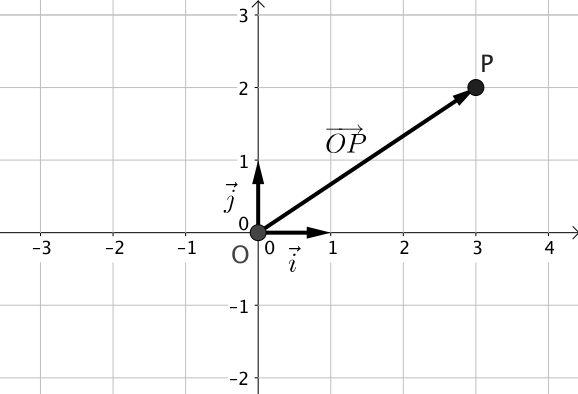
\includegraphics[width=0.23\textwidth]{img2/cartesian}
		\end{center}
	\end{wrapfigure}
	Per localitzar punts en el pla utilitzam un \textbf{sistema de referencia Cartesià} (en honor a René Descartes) format per:
 	 Un punt $O$ anomenat \textbf{origen}, i 
	  una \textbf{base} de vectors ortonormals $\vec i$, $\vec j$.
	 
	Qualsevol punt $P$ queda determinat mitjançant el \textbf{vector de posició} $\overrightarrow{OP}$.
\end{bluebox}
 \vspace{-0.5cm}
\begin{theorybox}[Punt mitjà d'un segment]
	Les coordenades del \textbf{punt mitjà, M,} d'un segment d'extrems $A(A_x, A_y)$ i $B(B_x, B_y)$ són:
	\begin{equation}
	M=\frac{A+B}{2} \,\,\,\,\,\, o \,\,\,\,\,\, M \left( \frac{A_x+B_x}{2},  \frac{A_y+B_y}{2} \right)
	\end{equation}
	
\end{theorybox}
\vspace{-0.5cm}

\begin{resolt}{Troba les coordenades dels punts que divideixen el segment $A(-2,5)$, $B(4,-1)$ en tres parts iguals.}
	Calculam el vector $\overrightarrow{AB}=B-A=(6,-6)$. Els punts seran:
	
	$A+\frac{1}{3}\overrightarrow{AB}=(-2,5)+(2,-2)=(0,3)$ i
	
	$A+\frac{2}{3}\overrightarrow{AB}=(-2,5)+(4,-4)=(2,1)$.
\end{resolt}

\begin{theorybox}[Punt simètric respecte d'un punt]
	\begin{wrapfigure}{R}{0.25\textwidth} 
		\vspace{-0.5cm}
		\begin{center}
			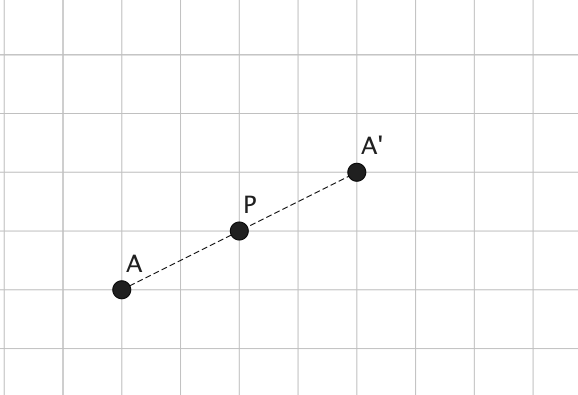
\includegraphics[width=0.23\textwidth]{img2/simetric}
		\end{center}
	\end{wrapfigure}
	Si volem calcular el \textbf{punt simètric $A'$} del punt $A$ respecte del punt $P$ raonam de la següent forma:
	El punt $P$ ha d'ésser el punt mitjà de l'interval $\overline{AA'}$ amb la qual cosa es compleix que  $P = \dfrac{A+A'}{2}$. Si aïllam $A'$ obtenim 
	\begin{equation*}
	A' = 2P-A \,\,\,\,\,\, o \,\,\,\,\,\,A' \left( 2P_x-A_x,  2P_y-A_y \right)
	\end{equation*}
	
\end{theorybox}

\vspace{-0.5cm}


\begin{resolt}{Troba el punt simètric de $A(2,-1)$ respecte del punt $P(-3,5)$}
	El simètric s'obté de $A' = 2P-A=2(-3,5)-(2,-1)=(-8, 11)$. Podeu comprovar que el punt mitjà de $A$ i $A'$ és $P$.
\end{resolt}



\begin{mylist}
	\item  Donats els punts $A=\left(1,4\right)$ i $B=\left(-3,6\right)$ calcula el seu punt mitjà.
	
	\item 
	\begin{minipage}{0.7\textwidth}
			Donats els punts $P(3,9)$ i $Q(8,-1)$
		\begin{tasks}
			\task Troba el punt mitjà del segment $PQ$
			\task El punt simètric de $P$ respecte de $Q$
			\task El punt simètric de $Q$ respecte de $P$
		\end{tasks}
	\end{minipage}	
	\begin{minipage}{0.3\textwidth}
		\vspace{-1cm}
	\begin{center}
		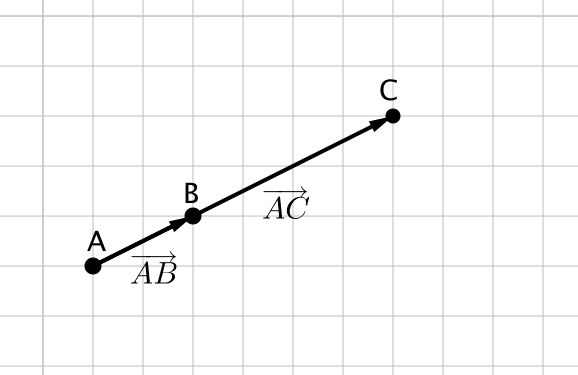
\includegraphics[width=0.8\textwidth]{img2/alineats}
	\end{center}
	
	\end{minipage}

 
	
\end{mylist}

\begin{theorybox}[Condició d'alineament de 3 punts]

	Tres punts $A(A_x, A_y)$, $B(B_x, B_y)$, $C(C_x, C_y)$ estan alineats si un parell de vectors $\overrightarrow{AB}$ i $\overrightarrow{AC}$ tenen igual direcció. Això passa si les components són proporcionals
	\begin{equation}
	\frac{B_x-A_x}{C_x-A_x}=\frac{B_y-A_y}{C_y-A_y}
	\end{equation}
\end{theorybox}


\begin{resolt}{Calcula el valor de $k$ perquè els punts $A(0,3)$, $B(-2, 5)$ i $C(4, k)$ estiguin alineats.}
	Calculam els vectors $\overrightarrow{AB}=B-A=(-2, 2)$ i $\overrightarrow{AC}=C-A=(4,k-3)$. Ara imposam que aquests dos vectors tinguin igual direcció; les components han d'ésser proporcionals.
	\begin{equation*}
	\frac{-2}{4}=\frac{2}{k-3}
	\end{equation*}
	Multiplicant en creu $-2(k-3)=8$ i d'aquí trobam que $k=-1$.
\end{resolt}




\begin{mylist}
		\item Calcula el valor de $k$ perquè els punts $A(1,7)$, $B(-3,4)$ i $C(k,5)$ estiguin alineats.
	
\end{mylist}


\section{Les equacions de la recta en el pla}


\begin{theorybox}
	L'equació de la recta que passa pel punt $P(P_x,P_y)$ i té vector director $\vec d=(d_x, d_y)$ es pot expressar de diferents formes:
	
	%\begin{multicols}{2}
	\textbf{Vectorial}: $(x,y)=(P_x,P_y)+\lambda (d_x, d_y)$ \vspace{0.25cm}
	
	\textbf{Paramètriques:} $\left\{ \begin{array}{l} x=P_x+ \lambda d_x \\ y=P_y+ \lambda d_y  \end{array} \right.$\vspace{0.25cm}
	
	\textbf{Contínua:} $\dfrac{x-P_x}{d_x}=\dfrac{y-P_y}{d_y}$\vspace{0.25cm}
	
	\textbf{Punt-pendent:} $y-P_y=m(x-P_x)$, essent \fbox{$m=\frac{d_y}{d_x}$} el pendent de la recta.\vspace{0.25cm}
	
	%\end{multicols}
	
	\textbf{Implícita o general:} $Ax+By+C=0$, essent $\vec n (A,B)$ el \textbf{vector normal} de la recta. $\vec d (-B,A)$ seria un vector director.\vspace{0.25cm}
	
	
	\textbf{Explícita:} $y=mx+n$, essent $m$ el pendent i $n$ l'ordenada a l'origen.
	
\end{theorybox}

\begin{resolt}{Escriu l'equació de la recta que passa pels punts $A(3,1)$ i $B(1,4)$ de totes les formes possibles.}
	Primer calculam el vector director de la recta $\vec d = \overrightarrow{AB}=(-2,3)$ i triam un dels punts, per exemple $A$.\vspace{0.25cm}
	
	L'equació vectorial és $(x,y)=(3,1)+\lambda(-2,3)$
	
	Les paramètriques són $\left\{ \begin{array}{l} x=3-2\lambda \\ y=1+3\lambda \end{array} \right.$
	
	L'equació contínua $\frac{x-3}{-2}=\frac{y-1}{3}$
	
	La punt-pendent $y-1 = -\frac{3}{2}(x-3)$
	
	La general $3x+2y-11=0$
	
	L'explícita $y=-\frac{3}{2}x+\frac{11}{2}$
	
\end{resolt}


\begin{mylist}
	\item Escriu l'equació de la recta que passa pel punts $A(1,-2)$ i $B(3,5)$ de totes les formes possibles.
	
	\item Obté un punt i un vector director de cadascuna d'aquestes rectes:
	\begin{tasks}(4)
		\task $\dfrac{x}{3}=\dfrac{y+1}{-2}$
		\task $y-2=4(x+7)$
		\task $x+y-2=0$
		\task $\left\{\begin{array}{l} x=2-3\lambda \\ y=2 \end{array}\right.$		
	\end{tasks}
	
	\item Obté un punt i un vector director de la recta $y=2x+5$ i expressa-la de totes les altres formes possibles.
	
 
\end{mylist} 

\hot Pàg. 36 -- Ex. 25; Pàg. 40 -- Ex. 15.
 

%%%%%%%%%%%%%%%%%%%%%%%%%%%%%%%%%%%%%%%%%%%%%%%%%%%%%%%%%%%%%%%%%%%%%%%%%%%%%%%%%%%%%%%%%%%%%%%
\section{Càlcul de la recta paral·lela i perpendicular}
\vspace{-0.25cm}
\begin{theorybox}[Segons vectors]
	Si ens donen una recta que té vector director $\vec d(d_x, d_y)$, per calcular
	\begin{itemize}
		\item una recta \textbf{paral·lela} a ella, utilitzam el \textbf{mateix vector} director (o proporcional).
		\item una recta \textbf{perpendicular} a ella, utilitzam el \textbf{vector normal}  $\vec n(-d_y, d_x)$.
	\end{itemize}
\end{theorybox}	
\vspace{-0.25cm}

\begin{theorybox}[Segons pendents]
	Si ens donen una recta que té pendent $m$, per calcular
	\begin{itemize}
		\item una recta \textbf{paral·lela} a ella, utilitzam el \textbf{mateix pendent}.
		\item una recta \textbf{perpendicular} a ella, utilitzam el pendent $m'=-\dfrac{1}{m}$.
	\end{itemize}
\end{theorybox}	

\begin{resolt}[E]{Calcula l'equació general de la recta perpendicular a $r:$ $\frac{x}{-2}=\frac{y+2}{1}$ que passa pel punt $P(1,1)$}
	La recta $r$ té com a vector director $\vec d_r=(-2,1)$. El seu vector normal és $\vec n=(1,2)$. L'equació de la recta que ens demanen en forma contínua 
	\begin{equation*}
	\frac{x-1}{1}=\frac{y-1}{2}
	\end{equation*}
	Si la multiplicam en creu la passam a forma general $2x-y-1=0$.
\end{resolt}
\vspace{-0.5cm}	
\begin{resolt}{Calcula l'equació general de la recta paral·lela a $r:$\linebreak $y-5=\frac{1}{2}(x+1)$ que passa per l'origen de coordenades.}
	La recta $r$ té com a pendent $m=1/2$, i la recta paral·lela tindrà el mateix pendent. L'únic que hem de fer és canviar el punt per l'origen $(0,0)$. L'equació punt-pendent serà:
	\begin{equation*}
	y-0=\frac{1}{2}(x-0)
	\end{equation*}
	Si passam a forma general trobam $x-2y=0$.
\end{resolt}

\hot Pàg. 40 -- Ex. 10, 11, 12; Pàg. 41 -- Ex. 30

\begin{comment}
\begin{mylist}
	
		
	\item  Calculau la recta que és paral·lela a $r$: $\frac{x-1}{2} =\frac{y-2}{3} $ i passa pel punt $\left(0,\; 1\right)$. Expressa-la almenys en tres formes i dibuixa-la.
	
	\item  Calculau la recta que és paral·lela a $r$: $2x-3y=0$ i passa pel punt $\left(1,\; 2\right)$. Expressa-la almenys en tres formes i dibuixa-la.
	
	\item  Calculau una recta perpendicular a $r:$ $y=2x-1$ que passi per $\left(2,\, \, -1\right)$. Expressa-la almenys en tres formes i dibuixa-la.
	
	\item  Calculau una recta perpendicular a $r:$ $x+2y=5$ que passi per $\left(2,\, \, 0\right)$. Troba el punt d'intersecció entre les dues rectes.
	
	\item  Calculau el punt simètric de $P(6,3)$ respecte la recta $r:$ $x+2y-2=0$.
	
\end{mylist}	
\end{comment}

\vspace{-0.5cm}
%%%%%%%%%%%%%%%%%%%%%%%%%%%%%%%%%%%%%%%%%%%%%%%%%%%%%%%%%%%%%%%%%%%%%%%%%%%%%%%%%%%%%%%%%%%%%%%
\section{Posició relativa de dues rectes}
\begin{theorybox}[Segons punts i vectors]
	Ens donen dues rectes en el pla $r$ i $s$ de les quals sabem un punt i un vector director. La posició relativa es determina de la següent forma:
	\begin{equation}
	\vec d_r,\, \vec d_s : \left\{
	\begin{array}{l}
	\text{Diferent direcció} \rightarrow \text{Secants} \\
	\text{Igual direcció}:\left\{
	\begin{array}{l}
	R \in s \rightarrow \text{Coincidents} \\
	R \notin s \rightarrow \text{Paral·leles}
	\end{array}
	\right.
	\end{array}
	\right.
	\end{equation}
\end{theorybox}

\vspace{-0.5cm}

\begin{theorybox}[Segons l'equació general]
	Donades les rectes $r: Ax+By+C=0$ i $s: A'x+B'y+C'=0$ en forma general, poden determinar la posició relativa:
	\vspace{-0.25cm}
	\begin{multicols}{3}
		$\dfrac{A}{A'}\neq \dfrac{B}{B'}$ 
		
		són secants.
		
		$\dfrac{A}{A'} = \dfrac{B}{B'} \neq \dfrac{C}{C'}$ 
		
		són paral·leles.
		
		$\dfrac{A}{A'} = \dfrac{B}{B'} = \dfrac{C}{C'}$ 
		
		són coincidents.
	\end{multicols}
\end{theorybox}	
 

\begin{resolt}[E]{Determina la posició relativa de les rectes i el punt de tall si existeix.
		\begin{equation*}
		r: \left\{ \begin{array}{l} x=1+2\lambda \\ y= 14 - \lambda \end{array}\right.
		\end{equation*}	
		\begin{equation*}
		s: \frac{x-2}{1}=\frac{y}{-5}
		\end{equation*}	
	}
	Els vectors directors de les rectes $\vec d_r = (2,-1)$ i $\vec d_s = (1,-5)$ tenen clarament diferent direcció, aleshores les rectes són secants.
	
	Per trobar el punt de tall, passam la recta $s$ a forma general $5x+y-10=0$. Tot seguit hi substituïm la $x$ i la $y$ de la recta $r$
	\begin{equation*}
	5(1+2\lambda)+(14-\lambda)-10=0
	\end{equation*}	
	Resolem aquesta equació de 1r grau i obtenim $\lambda=-1$. Si substituïm aquest valor dins la recta $r$, trobam el punt de tall $(-1,15)$.
\end{resolt}
\vspace{-0.5cm}
\begin{resolt}[E]{Per a quin valor de $k$ les rectes 
		\begin{eqnarray*}
			r: 2x+ky-1=0 \\
			s: 3x-y+5=0
		\end{eqnarray*}	
		seran paral·leles? Hi ha algun valor pel qual siguin coincidents?}
	
	Els vectors normals de les rectes són $\vec n_r=(2,k)$ i $\vec n_s=(3,-1)$. Perquè les rectes siguin paral·leles també ho han d'ésser els seus vectors normals. Aleshores
	\begin{equation*}
	\frac{2}{3}=\frac{k}{-1}
	\end{equation*}	
	Aïllam $k$ de l'equació i obtenim $k=-\frac{2}{3}$.
	
	Donat que 
	\begin{equation*}
	\frac{2}{3}\neq \frac{-1}{5}
	\end{equation*}	
	les rectes mai seran coincidents.
\end{resolt}

\hot Pàg. 36 -- Ex. 24; Pàg. 40 -- Ex. 13, 14

\begin{comment}
\begin{mylist}
	 
	\item  Siguin les rectes $r\equiv \left\{\begin{array}{l} {x=2+\lambda } \\ {y=1-2\lambda } \end{array}\right. $ i $s\equiv 2x+y=2$. Estudia la seva posició relativa i calcula els seus punts de tall si els hi hagués.
	
	
	\item  Siguin les rectes $r\equiv \left(1,\; 1\right)+\lambda \left(-1,\; 2\right)$ i $s\equiv x+y=3$. Estudia la seva posició relativa i calcula els seus punts de tall si els hi hagués.
	
	\item  Siguin les rectes $r\equiv \left(0,\; -2\right)+\lambda \, \left(1,\; 4\right)$ i $s\equiv 4x-y-2=0$. Estudia la seva posició relativa i calcula els seus punts de tall si els hi hagués. 
\end{mylist}	
\end{comment}


%%%%%%%%%%%%%%%%%%%%%%%%%%%%%%%%%%%%%%%%%%%%%%%%%%%%%%%%%%%%%%%%%%%%%%%%%%%%%%%%%%%%%%%%%%%	
\section{Distàncies}
\begin{theorybox}
	\textbf{Distància entre dos punts}: És igual al mòdul del vector que els uneix 
	\begin{equation*}
	d(A,B)=|\overrightarrow{AB}|=\sqrt{(B_x-A_x)^2 + (B_y-A_y)^2}
	\end{equation*}
	
	\textbf{Distància entre un punt i una recta}: Si el punt pertany a la recta la distància és zero. En cas contrari, suposem que la recta ve donada en forma general $Ax+By+C=0$. Aleshores, la distància s'obté de:
	\begin{equation*}
	d(P,r)=\frac{|A\,P_x+B\,P_y+C|}{\sqrt{A^2+B^2}} 
	\end{equation*}
	
	\textbf{Distància entre dues rectes}: Si les dues rectes són secants o coincidents la distància és zero. Si les rectes són paral·leles basta en calcular la distància d'un punt qualsevol de la recta $s$ a la recta $r$.
\end{theorybox}

\begin{theorybox}[Angle entre rectes]
	Per calcular l'angle que formen dues rectes $r$ i $s$ basta calcular l'angle que formen els seus vectors directors (o vectors normals). 
	\begin{equation*}
	\alpha = \arccos \dfrac{\vec d_r \cdot \vec d_s}{|\vec d_r|\, |\vec d_s|}
	\end{equation*}
\end{theorybox}

\begin{resolt}[E]{Per a quins valors de $k$ els punts $P(10,4)$ i $Q(1,k)$ es troben a distància 15 unitats?}
	La fórmula de la distància entre dos punts
	\begin{equation*}
	dist(P,Q)=\sqrt{(1-10)^2+(k-4)^2}=15
	\end{equation*}
	Si elevam al quadrat per eliminar l'arrel, arribam a l'equació de segon grau $81+(k-4)^2=225$ que té com a solucions $k=-8$ i $k=16$.
\end{resolt}
\vspace{-0.65cm}
\begin{resolt}{Calcula el punts sobre la recta $y=2x$ que distin 1 del punt $P(1,1)$.}
	Passam la recta a forma vectorial $(x,y)=(\lambda, 2\lambda)$. La fórmula de la distància entre dos punts
	\begin{equation*}
	dist(X,P)=\sqrt{(\lambda-1)^2+(2\lambda-1)^2}=1
	\end{equation*}
	Elevam al quadrat l'equació arribam a $5\lambda^2-6\lambda+1=0$. Aquesta equació de segon grau té dues solucions $\lambda=1$ i $\lambda=1/5$. Substituïnt cada valor de $\lambda$ dins la forma vectorial, trobam els punts de la recta $X_1=(1,2)$ i $X_2=(\frac{1}{5}, \frac{2}{5})$.
\end{resolt}
\vspace{-0.65cm}
\begin{resolt}{Calcula l'àrea del triangle de vèrtexs $A(-3,-2)$, $B(9, 7)$ i $C(2,8)$.
		
		\includegraphics[width=5cm]{img2/chap-anal-areat}
	}
	Necessitam calcular l'altura $h_C$. Per això, hem d'obtenir l'equació de la recta que passa per $A$ i $B$:\vspace{0.25cm}
	
	Pendent: $m=\frac{9}{12}=\frac{3}{4}$ $\rightarrow$ $y+2=\frac{3}{4}(x+3)$ $\rightarrow$ \fbox{$3x-4y+1=0$}\vspace{0.25cm}
	
	Altura: $h_c=dist(C, r_{AB})=\dfrac{|3\cdot 2-4\cdot 8+1|}{\sqrt{3^2+4^2}}=\frac{25}{5}=5$.\vspace{0.25cm}
	
	La base $c=dist(AB)=\sqrt{(9+3)^2+(7+2)^2}=15$\vspace{0.25cm}
	
	Àrea del triangle: $A=\dfrac{15\cdot 5}{2}=37.5\, u^2$
\end{resolt}
\vspace{-0.65cm}
\begin{resolt}{Troba un punt de l'eix de les abscisses que equidisti de les rectes $4x+3y+6=0$ i $3x+4y-9=0$.}
	
	Si el punt es troba l'eix de les abscisses serà de la forma $P(x,0)$. \vspace{0.25cm}
	
	Distància de $P$ a la 1a recta: $d_1 = \dfrac{|4x+6|}{\sqrt{4^2+3^2}}$\vspace{0.25cm}
	
	Distància de $P$ a la 2a recta: $d_2 = \dfrac{|3x-9|}{\sqrt{3^2+2^2}}$\vspace{0.25cm}
	
	Igualam les distàncies: $\dfrac{|4x+6|}{5}=\dfrac{|3x-9|}{5}$ \vspace{0.25cm}
	
	Aquesta equació amb valors absoluts té dues posibilitats $4x+6=3x-9$ o $4x+6=-(3x-9)$. Cada cas dóna una solució $x=-15$ i $x=3/7$. 
\end{resolt}

\begin{comment}

\begin{mylist}
	\item   Calcula la distància del punt (1, 2) a les rectes que s'indiquen.
	\begin{tasks}(2)
		\task $x+3y=4$   \task $\left\{\begin{array}{l} {x=1-\lambda } \\ {y=2+2\lambda } \end{array}\right. $  \task $\dfrac{x-1}{2} =\dfrac{y-3}{-1} $  \task $y-2=4\left(x+1\right)$
	\end{tasks}
	
	\item  Troba la posició relativa de les rectes $r{\rm :}\frac{x}{-{\rm 1}} =\frac{y+{\rm 3}}{-{\rm 1}} $ i
	$s{\rm :}\left(x,y\right)=\left({\rm 1,}\; -{\rm 2}\right)+\lambda \left({\rm 1,}\; {\rm 1}\right)$
	així com l'angle que formen.
	
	
	\item  Tres punts d'un triangle són  A = (2, 1), \textit{B} = (2, 8) i \textit{C} = (4, $-$1). Calcular els seus costats i angles. 
	
	
\end{mylist}
\end{comment}

\vspace{-0.5cm}

\hot Pàg. 36 -- Ex. 26, 29, 30, 31

\hot Pàg. 40 -- Ex. 19, 27, 28

\subsection{Rectes i punts notables d'un triangle}

\begin{theorybox}[Rectes notables]
	
	Considerau el costat AB d'un triangle de vèrtexs ABC:
	
	\begin{itemize}
		\item \textbf{Mediana}: És la recta que passa pel punt mitjà $M=\frac{A+B}{2}$ del segment i que passa pel vèrtex oposat $C$.
		
		\item \textbf{Altura}: És la recta que passa pel vèrtex oposat $C$ i que és perpendicular al segment $AB$.
		
		\item \textbf{Mediatriu}: És la recta que passa pel punt mitjà de $AB$ i que és perpendicular a ell.
		
		\item \textbf{Bisectriu}: Si $r_{AB}$ és la recta que passa per $AB$ i $r_{AC}$ la recta que passa per $AC$, la bisectriu és el lloc geomètric de tots els punts $X(x,y)$ que equidisten de les dues rectes.
		\begin{equation*}
		dist(X,r_{AB}) = dist(X,r_{AC})
		\end{equation*}
	\end{itemize}
	
	
	\begin{center}
		
		\includegraphics[height=3.cm]{img2/mediana.png}
		\includegraphics[height=3.cm]{img2/altura.png}
		\includegraphics[height=3.cm]{img2/mediatriu.png}
		\includegraphics[height=3.cm]{img2/bisectriu.png}
		
	\end{center}
\end{theorybox}


\begin{theorybox}[Punts notables]
	Considerau un triangle de vèrtexs ABC:
	
	\begin{itemize}
		\item \textbf{Baricentre (G)}: és el punt on es tallen les medianes. Representa el centre de gravetat del triangle.
		\item \textbf{Ortocentre (H)}: és el punt on es tallen les altures. 
		\item \textbf{Circumcentre (O)}:  és el punt on es tallen les mediatrius. És el centre de la circumferència circumscrita en el triangle.
		\item \textbf{Incentre (I)}: és el punt on es tallen les bisectrius. És el centre de la circumferència inscrita en el triangle.
	\end{itemize}
	\begin{center}
		
		
		\includegraphics[height=2.7cm]{img2/baricentre.png}
		\includegraphics[height=2.7cm]{img2/ortocentre.png}
		\includegraphics[height=2.7cm]{img2/circumcentre.png}
		\includegraphics[height=2.7cm]{img2/incentre.png}
		
	\end{center}
	
\end{theorybox}

\hot Pàg. 37 -- Ex. 34, 36, 38

\begin{comment}

\begin{mylist}
	
	\item  \hot Donat el triangle de vèrtexs \textit{ABC}, essent  A = (0, 0), \textit{B} = (6, 0) i \textit{C} = (4, 4), determina les equacions de:
	\begin{enumerate}
		\item  Les seves mediatrius i les coordenades del circumcentre
		
		\item  Les seves bisectrius i les coordenades de l'incentre
		
		\item  Les seves altures i les coordenades de l'ortocentre
		
		\item  Les seves mitjanes i les coordenades del baricentre
	\end{enumerate}
\end{mylist}


%%%%%%%%%%%%%%%%%%%%%%%%%%%%%%%%%%%%%%%%%%%%%%%%%%%%%%%%%%%%%%%%%%%%%%%%%%%%%%%%%%%%%%%%%%%%%%%%%%%%%%%%%%%%	
\begin{activitats}
	
	\begin{mylist}	
		
		\item  Considerem la recta  $r\equiv \frac{x-1}{-1} =\frac{y-2}{3} $. 
		
		\begin{enumerate}
			\item  Calcula el seu pendent.
			
			\item  Pertany el punt $\left(0,\, \, 5\right)$ a la recta? I el $\left(1,\; 3\right)$?
			
			\item  Dóna almenys tres punts de la recta.
			
			\item  Dibuixa la recta.
		\end{enumerate}
		
		\item  Siguin els punts \textit{A =} (1, 2) i \textit{B} = (3, 0)
		\begin{enumerate}
			\item  Calcula el vector que els uneix.
			
			\item  Calcula l'equació general de la recta que passa per tots dos.
			
			\item  Pertany el punt (2, 1) a la recta?, i el (3, 1)?
		\end{enumerate}
		
		
		\item  Considerem la recta $y-2x=1$
		
		\begin{enumerate}
			\item  Calcular el seu pendent i vector director.
			
			\item  Dóna una recta perpendicular a ella que passi per (1, 2). Expressa-la almenys de quatre formes.
		\end{enumerate}
		
		
		
		\item  Sigui la recta $r\equiv y=x-2$.
		
		\begin{enumerate}
			\item  Calcula una recta perpendicular a ella i passada per (2, 1).
			
			\item  Calcula una recta que passi per (--1, 3) i sigui paral·lela a  $r$ .
		\end{enumerate}
		
		\item  Troba la posició relativa de les rectes $x+y=0$ i $s\equiv \left(x,y\right)=\left(1,\; 2\right)+\lambda \left(1,\, \; 1\right)$ així com l'angle que formen.
		
		\item  Suposa que la distància d'un punt a una recta és 0. Què significa aquest resultat? Aplica-ho a la recta $2x-y=1$ i el punt (2, 3).
		
		\item  Sigui la recta $s:\, x+y=4$. 
		\begin{enumerate}
			\item  Calcula una recta perpendicular amb ella i passada per (1, 1). 
			
			\item  Calcula la distància d'aquesta recta al punt (2, 3).
		\end{enumerate}
		
		
		
		
		\item  Sigui la recta $s{\rm :}x-{\rm 2y}+{\rm 1}={\rm 0}$ 
		
		\begin{enumerate}
			\item  Calcula una recta que sigui perpendicular a ella i passada per (1, 1).
			
			\item  Calcula una recta que passi per (0, 1) i sigui paral·lela a  s .
		\end{enumerate}
		
		
		\item  Tres punts d'un rectangle \textit{ABCD} són \linebreak \textit{A} = (2, 1), \textit{B}= (0, 7) i \textit{D} = (5, 2). Es demana:
		\begin{enumerate}
			\item  Calcular el punt \textit{C}.
			
			\item  Comprovar que l'angle \textit{B} és de 90º.
			
			\item  Calcular les longituds dels costats \textit{AB}, \textit{BD} i \textit{CD} del rectangle.
			
		\end{enumerate}
		
		
		
		
		\item  Troba la posició relativa de les rectes $r:\, 3x+y=5$ i $s:\, \left(x,y\right)=\left(1,-2\right)+\lambda \left(-1,3\right)$ així com l'angle que formen.
		
		\item  Calcula la recta perpendicular a \linebreak $y=2x-4$  que passi pel punt mitjà de \textit{A} = (1, 3) i \textit{B} = (3,-1)
		
		
		\item  Calcula la distància a l'origen de les rectes que s'indiquen.
		\begin{tasks}(2) 
			\task $2x+y=3$  \task  $y=\dfrac{x}{2} $ \task*(2)  $\left(x,y\right)=\left(1,\; -2\right)+\lambda $ 
		\end{tasks}
		
		
		\item  Calcula la distància del punt (2, $-$1) a la recta $y+x=1$. 
		
		\item  Calcula la distància al punt (1, $-$2) de les següents rectes.
		\begin{tasks}(2)
			\task $\left\{\begin{array}{l} {x=1+\lambda } \\ {y=-\lambda } \end{array}\right. $   \task $2x+y=3$ 
		\end{tasks}
		
		
		\item  Calcula la distància del punt (1, 4) a la recta $y-x=1$ 
		\item  Una recta passa pel punt (3, 1) i forma amb els semieixos positius un triangle d'àrea 6 unitats. Calcula l'equació d'aquesta recta.
		
		\item  Calcula el punt de simètric de $A=(1, 2)$ respecte a la recta $y=3$.
		
		\item  Considerem un pentàgon irregular \textit{ABCDE} format pels punts 
		\textit{A =} ($-$2, 3),  \textit{B} = (1, 4), \textit{C }= (3,3), \textit{D} = (2, 2) i \textit{I} = ($-$1, 1). 
		Dibuixa-ho i calcula la seva àrea.  Et recomanem dividir-ho en figures més manejables.
		
		
		\item  Considerem un quadrat \textit{ABCD}. El punt \textit{A} és (1, 2) i els punts \textit{B} i \textit{C} estan sobre la recta $y-x=3$. Calcula els quatre vèrtexs del quadrat i la seva àrea.
		
		
		
		\item  Determina les mediatrius dels segments d'extrems \textit{A} i \textit{B}. Representa-ho gràficament.
		\begin{tasks}
			\task \textit{A =} (0, 7) i \textit{B} = (0, 3)   \task \textit{A =} (--3, 0) i \textit{B} = (6, 0)   \task\textit{A =} (--5, 0) i \textit{B} = (0, --5)
		\end{tasks}
		
		\item  Determina les bisectrius de les rectes $r$ i $s$ per cada un dels casos següents. Representa-ho gràficament.
		\begin{tasks}
			\task $r: \, x+2y-5=0$ i
			
			$s: \, 2x-y-8=0$
			\task $r: \, 3x+5y-2=0$ i 
			
			$s: \, 4x-6y-1=0$
			\task $r: \, x=0$ i $s: \,y=0$
			\task $r: \, x+y=0$ i $s: \, x-y=0$
		\end{tasks}
		
		
		\item  Considera la recta $x+2y=3$ i el punt $A(2, 3)$. Calcula el punt \textit{Q} de mínima distància i el simètric de  \textit{A} respecte de la recta.
		
		
		
		\item  En un paral·lelogram \textit{ABCD}, els vèrtexs venen donats per \textit{A} = (1, 1), \textit{B}= (2, 3) i \textit{C}= 3, $-$1).
		\begin{enumerate}
			\item  Calcula l'angle $\hat B$ (entre els costats \textit{BA} i \textit{BC}).
			
			\item  Calcula l'equació de la recta que passa per \textit{A} i \textit{C} (la diagonal del paral·lelogram).
			
			\item  Calcula el perímetre de la figura.
			
			\item  Calcula el punt \textit{D}.
		\end{enumerate}
		
		\item  Ja saps que la mediatriu és el lloc geomètric dels punts que equidisten de dos punts donats. Escriu l'equació de la mediatriu del segment d'extrems \textit{A}=(2, 5) i \textit{B}=(4, $-$1).
		
		\item  Recordem que el circumcentre d'un triangle és el punt de tall de les mediatrius dels seus costats. Calcula el circumcentre del triangle \textit{A =} (1, 2), \textit{B} = (1, 6) i \textit{C} = (3, 8) escrivint les equacions de les tres mediatrius.
		
		\item  Recordem que el baricentre d'un triangle és el punt d'intersecció de les mitjanes (la mitjana és la recta que va des d'un vèrtex al punt mitjà del costat oposat). Sabent això, calcula el baricentre del triangle \textit{A}=($-$2, 2), \textit{B}=(1, 4) i \textit{C} = (1, 0), escrivint les equacions de les tres mitjanes.
		
		\item  Ja saps que la bisectriu d'un angle és el lloc geomètric dels punts que equidisten dels costats de l'angle. Escriu l'equació de la bisectriu de l'angle format per les rectes \textit{y} = 2\textit{x} + 3, i 3\textit{x} + 5\textit{y} = 1. Quantes hi ha? Com són?
	\end{mylist}	
	
\end{activitats}	

\autoaval
\begin{enumerate}
	\item Es consideren els punts $A(0,1)$, $B(4,9)$ i $C(-4,k)$. Troba $k$ perquè
	\begin{tasks}
		\task Els punts estiguin alineats.
		\task Perquè el punt $C$ sigui el punt simètric de $B$ respecte $A$.
	\end{tasks}
	
	\item Calcula l'equació de les rectes:
	\begin{tasks}
		\task Que passa per $A(3,2)$ i $B(-2,1)$ en forma contínua i general.
		\task Que passa per $A(1,1)$ i té pendent $-3$ en forma punt-pendent i general.
	\end{tasks}
	
	\item Calcula l'equació de les rectes:
	\begin{tasks}
		\task Passa per $P(2,-3)$ i és perpendicular a $(x,y)=(0,1)+t(5,-2)$.
		\task És paral·lela a $2x+3y+1=0$ i passa pel punt $(0,2)$.
	\end{tasks}
	
	\item Estudia la posició relativa de les rectes $r$ i $s$ segons els valors del paràmetre $k$
	$r: \, 3x+ky-34=0$ i $s: \, y=\frac{5}{3}x$.	
	
	
	\item  Calcula $k$ perquè les rectes $y=3$ i $y=kx+1$ formin un angle de $60^\circ$.
\end{enumerate}

\end{comment}

\end{document}